\documentclass[border=10pt]{standalone}
\usepackage{tikz}
\usetikzlibrary{shapes, arrows.meta, positioning}

\definecolor{espsoft}{HTML}{4A904A}
\definecolor{actred}{HTML}{D94A4A}

\tikzset{
    state/.style={rectangle, draw, fill=white, minimum width=1.5cm, minimum height=0.7cm, align=center, font=\small, rounded corners=2pt},
    staterun/.style={state, fill=green!15, draw=espsoft},
    stateerr/.style={state, fill=red!15, draw=actred},
    stateidle/.style={state, fill=gray!10, draw=gray},
    arr/.style={-{Stealth[length=2mm]}, thick},
    arrlab/.style={font=\scriptsize, fill=white, inner sep=1pt},
}

\begin{document}
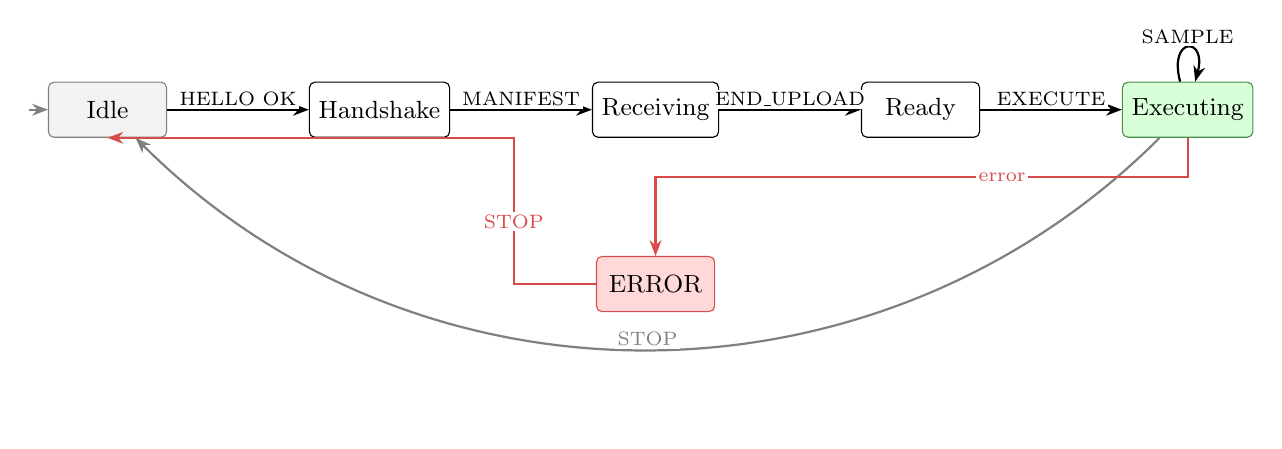
\begin{tikzpicture}[node distance=1.8cm]

% ── Main flow (horizontal) ──
\node[stateidle] (idle) at (0, 0) {Idle};
\node[state, right=of idle] (hs) {Handshake};
\node[state, right=of hs] (recv) {Receiving};
\node[state, right=of recv] (ready) {Ready};
\node[staterun, right=of ready] (exec) {Executing};

% ── ERROR (below center) ──
\node[stateerr, below=1.5cm of recv] (err) {ERROR};

% ── Start ──
\draw[arr, gray] (-1, 0) -- (idle);

% ── Forward flow ──
\draw[arr] (idle) -- node[arrlab, above] {HELLO OK} (hs);
\draw[arr] (hs) -- node[arrlab, above] {MANIFEST} (recv);
\draw[arr] (recv) -- node[arrlab, above] {END\_UPLOAD} (ready);
\draw[arr] (ready) -- node[arrlab, above] {EXECUTE} (exec);

% ── STOP back (above) ──
\draw[arr, gray, bend left=45] (exec) to node[arrlab, above] {STOP} (idle);

% ── ERROR path (below) ──
\draw[arr, actred] (exec.south) -- ++(0,-0.5) -| node[arrlab, pos=0.2, right] {error} (err);
\draw[arr, actred] (err) -- ++(-1.8,0) |- node[arrlab, pos=0.25, below] {STOP} (idle.south);

% ── Loop ──
\draw[arr] (exec) to[loop above] node[arrlab] {SAMPLE} (exec);

\end{tikzpicture}
\end{document}
